

%В работе был рассмотрен ?вопрос проектировки? беспилотного летательного аппарата (БПЛА), предназаченного для длительного ($\approx24$~часа без дозаправки) барражирования в целях мониторинга и разведки (ограничения по режимам полета представлены на Рис.\ref{fig:ModeOfFlight}). В связи с этим к БПЛА были предъявлены высокие требования по малозаметности и аэродинамическому качеству. 




За основу гипотетической конструкции БПЛА была взята разработанная в ЦАГИ конструкция БПЛА, хорошо отвечающая требованиям высокого аэродинамического качества и требованиям малозаметности. Внешний вид гипотетической конструкции БПЛА показан на Рис.\ref{fig:BPLA_TSAGI}.
 

%Возможно, вставить пункт с геометрическими ограничениями
  
  



\begin{figure}[ht]
\centering
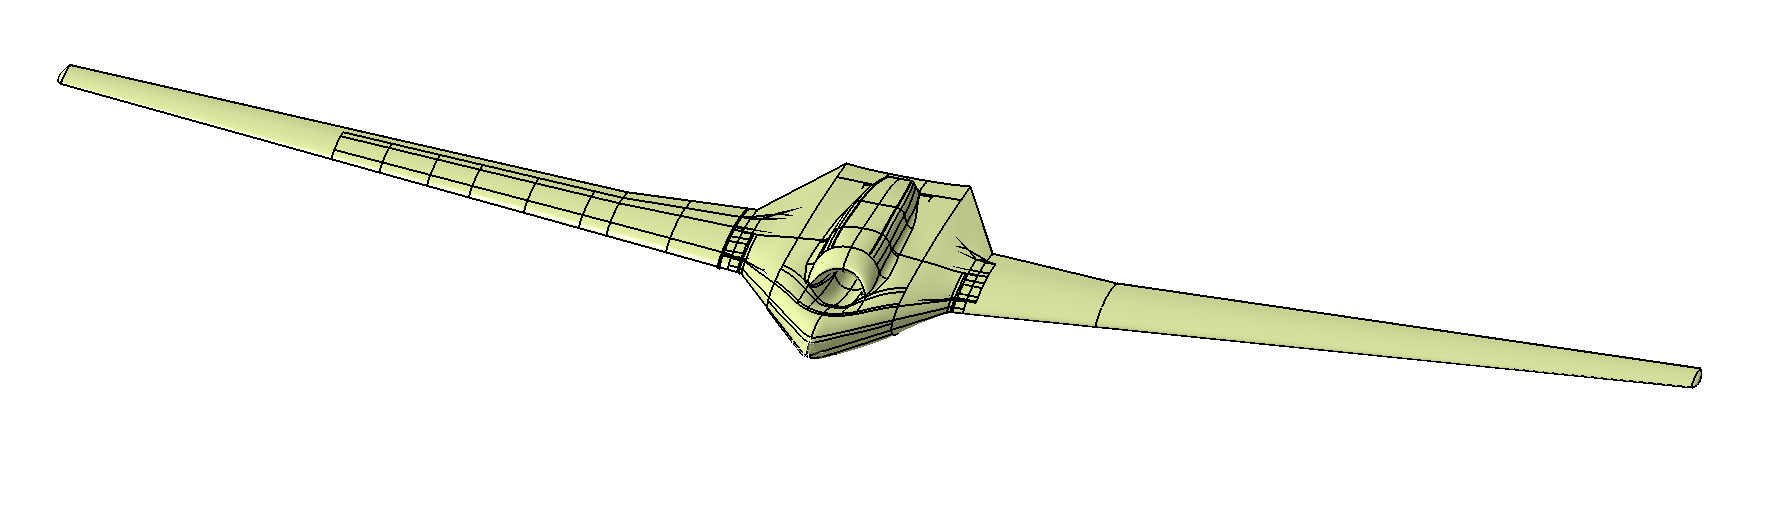
\includegraphics[width=1\textwidth]{BPS_Catia_Full}
\caption{Внешний вид гипотетической конструкции БПЛА}
\label{fig:BPLA_TSAGI}
\end{figure}

Конструкция выполнена по схеме ``бесхвостка'' с крылом большого удлинения и высокой степенью интегрированности крыла с фюзеляжем и двигателя с фюзеляжем. 

Для лучшей интеграции двигателя, включая воздухозаборник, в конструкцию БПЛА разработчикам пришлось использовать центроплан изогнутой формы (Рис.\ref{fig:OriginalSectionWithEngine}). Использование такой формы центроплана сопряжено с возможным возникновением новых проблем обеспечения прочности такого типа конструкции. Проблемы прочности в этом случае усугубляются из-за больших величин изгибающего момента, приходящего от крыла большого удлинения. 

Поскольку использование изогнутого центроплана может существенно ухудшить весовую эффективность БПЛА по сравнению с использованием прямого центроплана, для оценки величин этих весовых издержек необходимо проведение комплексных исследований по зависимости веса конструкции центроплана от геометрических параметров, характеризующих его кривизну. 
Необходимость таких исследований была связана с тем, что рассматриваемая в работе конструкция центроплана является нетрадиционной, и проведенный автором поиск конструкций прототипов не обнаружил наличия прямых прототипов данной конструкции центроплана для рассматриваемой размерности.

%Исследований центропланов такой формы ранее не проводилось.
 
%очевидно, что волнообразный центроплан может иметь напряжные вопросы с обеспечением прочности, т.к. такие центропланы в такой размерности не использовались, довольно нагружены. Сказать про компоновку, нарисовать её (общие вещи).

%с самого начала пишем, какие проблемы. Так сделали, такая компоновка, но у неё такие-то проблемы след волнообразный центроплан

%дальше: это может существенно ухудшить компоновку и весовую эффективность по сравнению с прямым центропланом. Цель работы - оценить возможные ухудшения. 

% и уже для того, чтобы оценить: следующий параграф 

Для оценки возможных ухудшений весовой эффективности конструкции центроплана необходимо построение расчетной прочностной модели гипотетической конструкции БПЛА, позволяющей проводить параметрический анализ зависимости прочности центроплана от геометрических параметров, определяющих его кривизну. Это необходимо и для последующего решения многодисциплинарной проектировочной задачи, в рамках которой будет возможность варьирования внешних аэродинамических обводов. 
Решение такой задачи предполагается осуществить в дальнейшем вне рамок данной работы. 

В настоящей (бакалаврской) работе не предполагается вариации внешних аэродинамических обводов и выхода этих параметров за пределы, определенные компоновкой "БПЛА-ЦАГИ", для которой они были выбраны из условия максимальной величины аэродинамического качества и минимума заметности, однако без учета требований прочности. 

%При построении модели необходимо было учесть ее дальнейшую модификацию, позволяющую варьировать форму внешних аэродинамических обводов. В бакалаврской работе форма внешних аэродинамических обводов постоянны. 


%Это скажем в разделе про нагрузки: Также постоянными считаются нагрузки на конструкцию (см.Раздел \ref{sec:externalLoads}). 

%В бакалаврской работе будем рассматривать только те обводы, которые есть в этой модели. И целью работы будет оценка потерь из-за такого центроплана (в прочности)

 
  
  

%Не забыть про то, что мы также хотим менять аэродинамику
%Требования: БПЛА, полет на таких-то высотах, столько-то. Весовая сводка такая-то, максимальные перегрузки, коэффициент запаса, аэродинамика. Ограничения - малозаметность, вес, пожаробезопасность отсека двигателя. 
%

